% ═══════════════════════════════════════════════════════════════════════════════
\section{Institutional Readiness for GVC Integration}
\label{sec:institutional}
% ═══════════════════════════════════════════════════════════════════════════════

\subsection{Analytical Framework: Institutions as GVC Entry Conditions}

The GVC literature increasingly recognises that institutional quality is not merely a background condition for development but a proximate determinant of whether FDI translates into domestic capability accumulation. Kaplinsky and Morris (2001) argue that GVC participation requires a minimum institutional threshold: functioning contract enforcement (so that supplier relationships are credible), property rights protection (so that technology-intensive firms will invest), and regulatory predictability (so that investors can plan multi-year production schedules). Below this threshold, FDI flows are possible but tend to be confined to extractive or infrastructure modes that generate enclave economies rather than integrated production networks.

Gereffi and Lee (2016) elaborate this point in the context of GVC governance: firms selecting between ``captive'' and ``relational'' governance arrangements will gravitate toward captive (controlling) arrangements in markets where institutional quality is weak, precisely because they cannot rely on contract enforcement and information asymmetries are high. This creates a self-reinforcing trap: low institutional quality attracts only captive GVC arrangements, which generate limited technology transfer and thus limited institutional upgrading. Breaking this trap requires institutional reform that is visible, credible, and verifiable to potential partners.

For Uzbekistan, this framework predicts that the institutional constraints documented below are not merely inconveniences but structural determinants of the \textit{type} of GVC integration that is achievable. As long as Uzbekistan scores below the regional median on governance indicators, it will attract infrastructure-linked investment (which requires less institutional trust, since assets are physical and observable) but will struggle to attract the relational manufacturing investment of the Japanese and Korean type that drove Vietnamese upgrading.

\subsection{World Governance Indicators: Uzbekistan in Comparative Perspective}

Figure~\ref{fig:wgi_comparison} presents Uzbekistan's percentile scores on six World Bank Governance Indicators (WGI) for 2023 and compares them to Vietnam and Thailand at their respective six-year-post-reform stages and to the global median.

\begin{figure}[H]
 \centering
 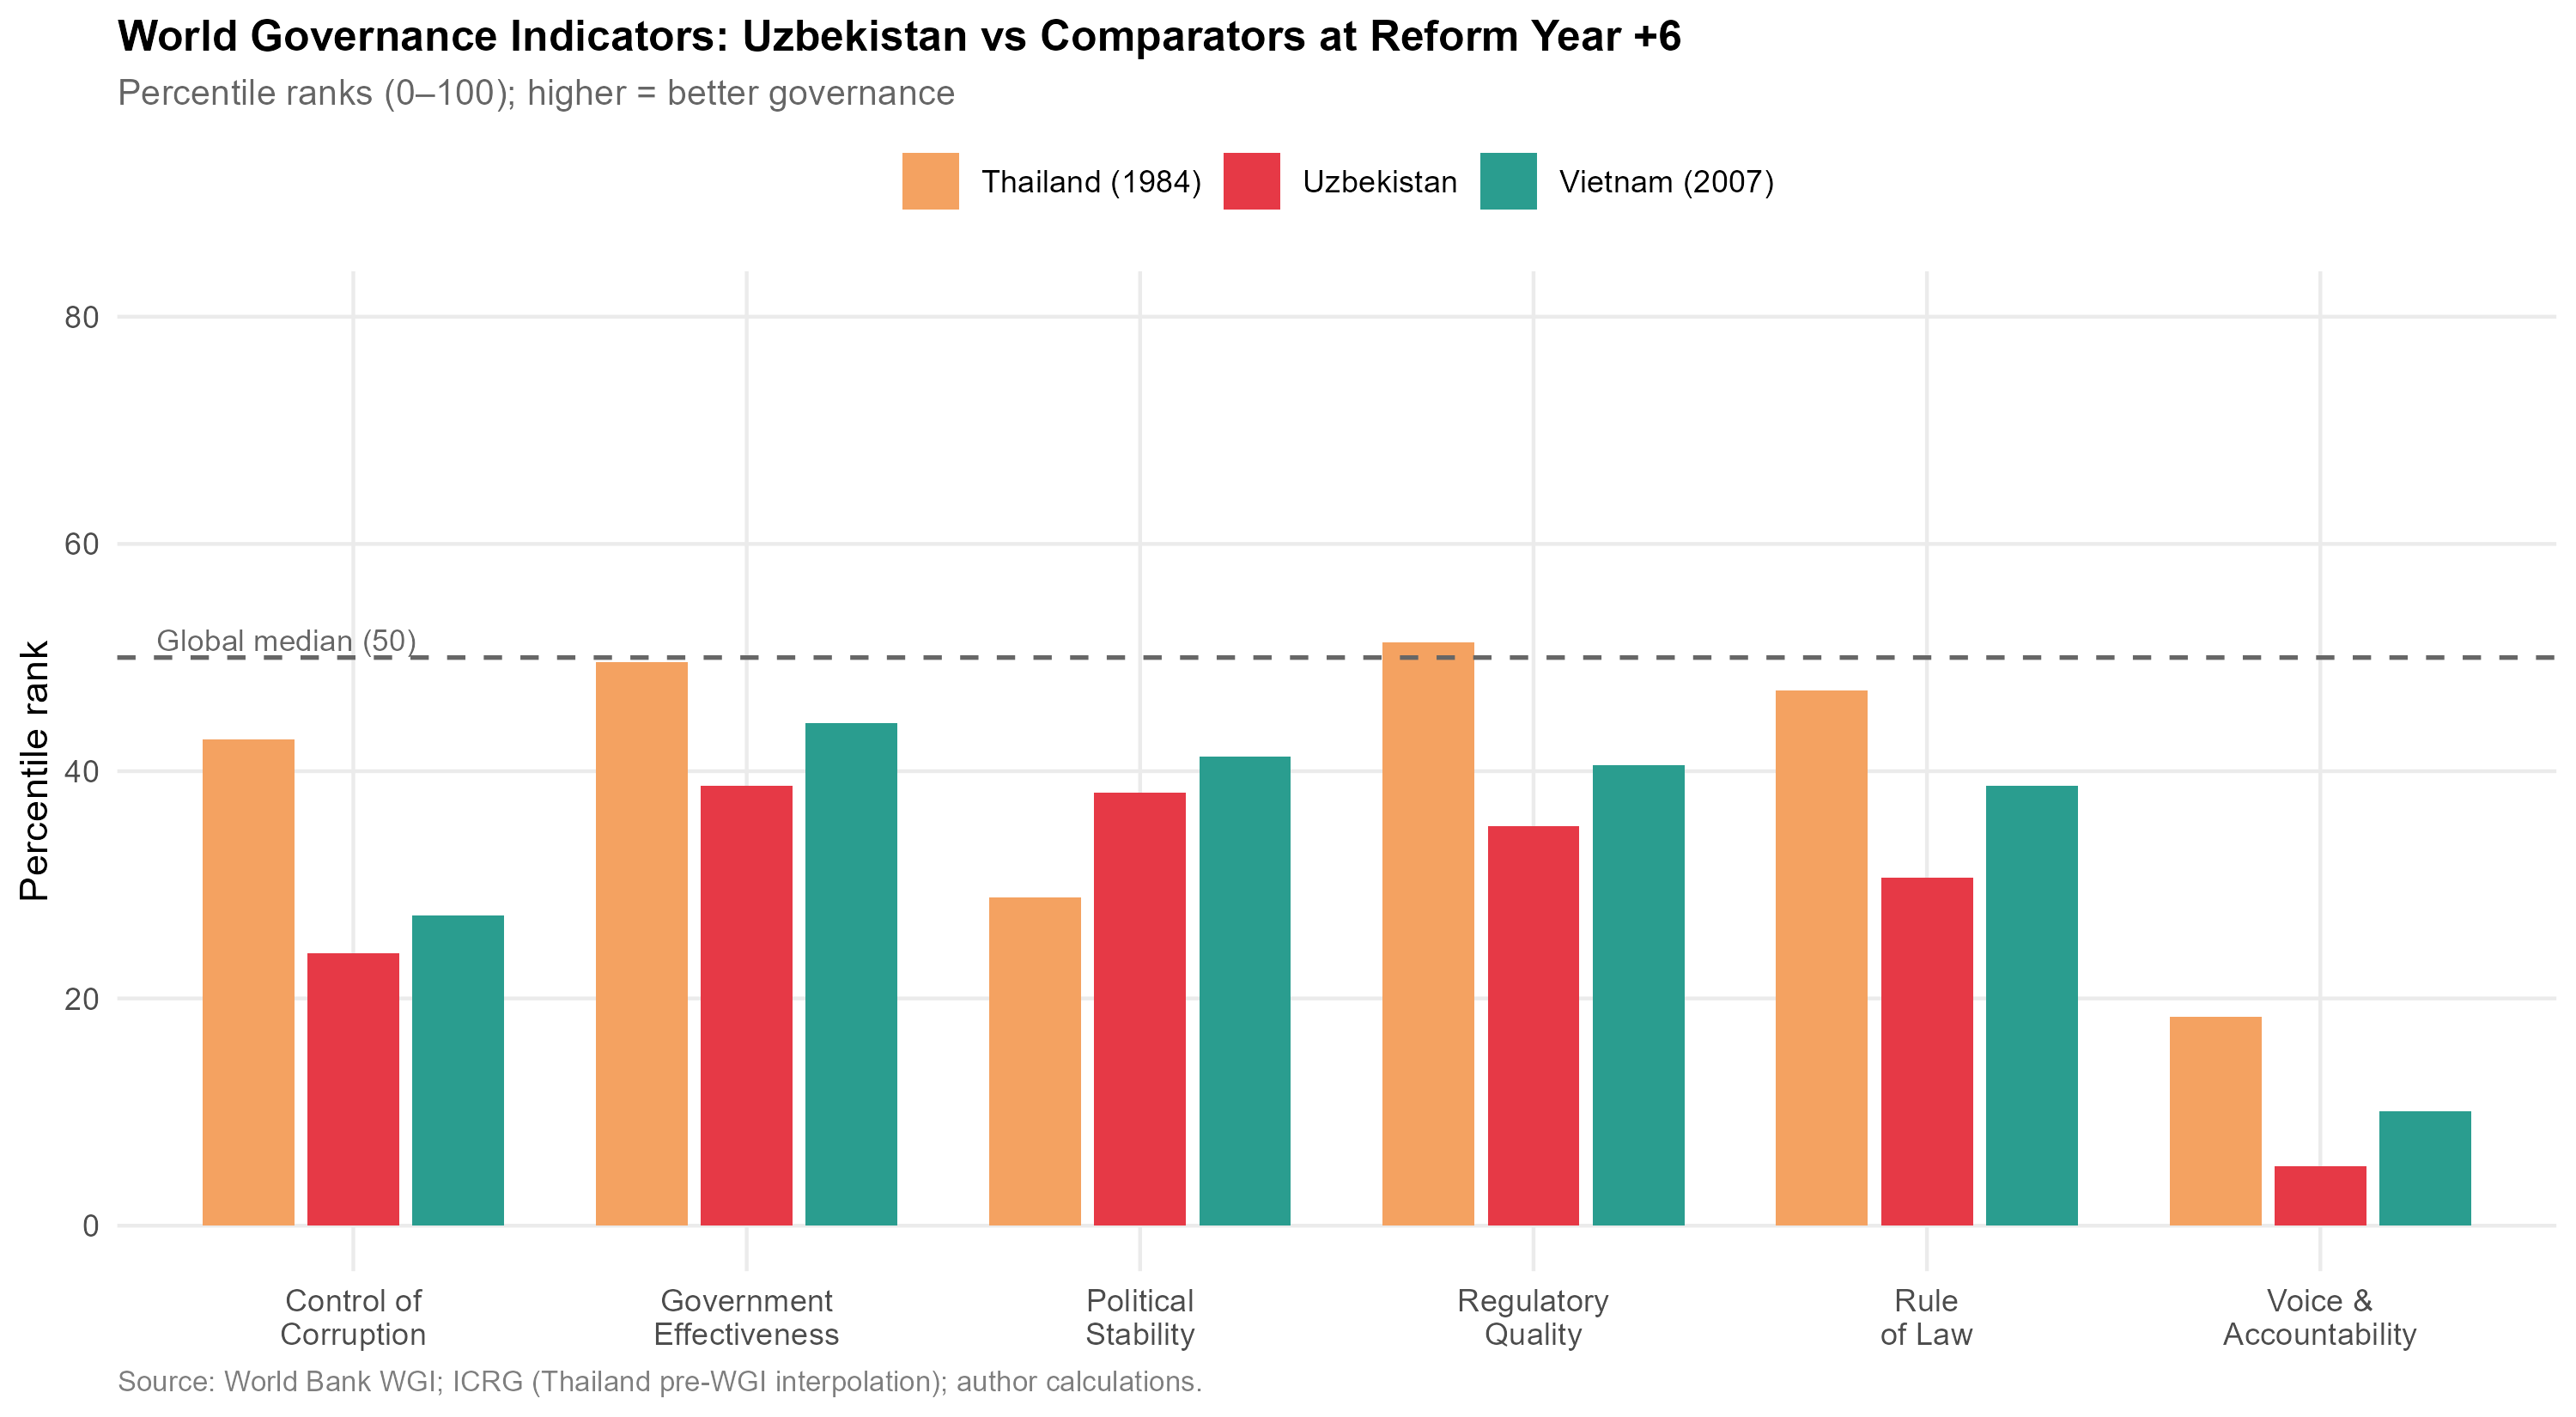
\includegraphics[width=0.92\textwidth]{figures/fig18_wgi_comparison.png}
 \caption{World Governance Indicators: Uzbekistan (2023) vs.\ Vietnam (2007) and Thailand (1984) at comparable reform stages. Scores are country percentile ranks (0--100); higher is better. Global median = 50. Source: World Bank WGI; pre-WGI Thailand values interpolated from ICRG political risk indices.}
 \label{fig:wgi_comparison}
\end{figure}

\begin{table}[H]
 \centering
 \caption{World Governance Indicators: Comparative Percentile Ranks}
 \label{tab:wgi}
 \small
 \begin{tabular}{@{}lcccc@{}}
 \toprule
 WGI Dimension & Uzbekistan 2023 & Vietnam 2007 & Thailand 1984* & Global Median \\
 \midrule
 Voice \& Accountability & 5.2 & 10.1 & 18.4 & 50.0 \\
 Political Stability & 38.1 & 41.3 & 28.9 & 50.0 \\
 Government Effectiveness & 38.7 & 44.2 & 49.6 & 50.0 \\
 Regulatory Quality & 35.2 & 40.5 & 51.3 & 50.0 \\
 Rule of Law & 30.6 & 38.7 & 47.1 & 50.0 \\
 Control of Corruption & 24.0 & 27.3 & 42.8 & 50.0 \\
 \midrule
 \textbf{WGI Composite (mean)} & \textbf{28.6} & \textbf{33.7} & \textbf{39.7} & \textbf{50.0} \\
 \bottomrule
 \end{tabular}
 \\\smallskip
 \small * Pre-WGI Thailand estimates interpolated from ICRG Risk Ratings; Vietnam 2007 from World Bank WGI database. All values are percentile ranks (0--100). Source: World Bank Governance Indicators; ICRG; author calculations.
\end{table}

Table~\ref{tab:wgi} reveals a consistent pattern: Uzbekistan at reform year +6 (2023) scores approximately 5--10 percentile points below Vietnam at reform year +6 (2007) on every governance dimension except Political Stability. The gaps are largest in Control of Corruption (6-point deficit) and Rule of Law (8-point deficit) --- precisely the dimensions most critical for manufacturing investment decisions, since they determine the reliability of supplier contracts and the security of proprietary technology brought by investing firms.

The comparison with Thailand (1984) is more complex, as Thailand's institutional environment at that stage was shaped by a different post-colonial history and a more stable bureaucratic tradition. However, even Thailand scored above Uzbekistan on Regulatory Quality and Government Effectiveness, suggesting that there is nothing structurally inevitable about the current gap: it reflects current policy choices rather than irreversible institutional legacies.

\subsection{Regulatory Quality: Investment Climate Dimensions}

The World Bank's B-READY (Business Ready) Index, which replaced Doing Business in 2023, offers a more granular picture of regulatory quality relevant to manufacturing investment. Table~\ref{tab:bready} presents Uzbekistan's scores on dimensions most critical for export-oriented manufacturing FDI.

\begin{table}[H]
 \centering
 \caption{Selected B-READY / Doing Business Indicators: Uzbekistan and Comparators}
 \label{tab:bready}
 \small
 \begin{tabular}{@{}lccc@{}}
 \toprule
 Indicator & Uzbekistan 2023 & Vietnam 2023 & Thailand 2023 \\
 \midrule
 Starting a Business (days) & 7 & 6 & 5 \\
 Registering Property (days) & 11 & 57 & 7 \\
 Trading Across Borders: Export (hrs) & 89 & 48 & 18 \\
 Trading Across Borders: Import (hrs) & 112 & 55 & 14 \\
 Enforcing Contracts (days) & 290 & 400 & 420 \\
 Resolving Insolvency (years) & 2.8 & 2.0 & 1.5 \\
 Getting Electricity (days) & 25 & 31 & 37 \\
 \bottomrule
 \end{tabular}
 \\\smallskip
 \small Source: World Bank B-READY 2023; World Bank Doing Business 2020 (Vietnam/Thailand). Uzbekistan Doing Business data from last available survey (2020) where B-READY not yet published.
\end{table}

Two dimensions stand out. First, trading across borders --- the most directly relevant indicator for export-oriented manufacturing --- shows Uzbekistan's border crossing time for exports (89 hours) nearly double Vietnam's (48 hours) and five times Thailand's (18 hours). This is not merely a bureaucratic inconvenience: a 71-hour additional delay per export shipment, compounded across a supply chain requiring regular just-in-time component delivery, can render time-sensitive manufacturing economically unviable regardless of labour cost advantages.

Second, contract enforcement time (290 days) is notably shorter than Vietnam (400 days) and Thailand (420 days), suggesting that Uzbekistan's judicial system, while weak on independence (as captured in Rule of Law), is relatively efficient in processing commercial disputes. This represents an underappreciated institutional asset that should be emphasised in investment promotion.

\subsection{Investment Treaty Architecture}

A country's bilateral investment treaty (BIT) network constitutes a credible commitment device that reduces political risk for foreign investors by establishing international arbitration mechanisms, national treatment guarantees, and protections against expropriation. UNCTAD's Investment Policy Framework records Uzbekistan as party to 49 BITs in force as of 2023, compared to Vietnam (66 BITs) and Thailand (41 BITs). Uzbekistan's BIT coverage is therefore not systematically inferior to Thailand's, though it is weaker than Vietnam's.

However, the quality and enforceability of BITs matters as much as quantity. Several of Uzbekistan's BITs --- including those with China, Russia, and several Gulf states --- were concluded before 2010 under outdated templates that lack investor-state dispute settlement (ISDS) provisions consistent with modern standards (UNCITRAL Rules 2013, ICSID Convention). The absence of a functioning double-taxation treaty (DTT) with Japan until 2023 represented a particular deterrent to Japanese manufacturing investment, as Japanese conglomerates' corporate treasury departments treat DTT coverage as a threshold requirement for long-term equity investment. The Japan-Uzbekistan DTT signed in 2023 is therefore a significant institutional development that post-dates the period of this analysis but should be monitored as a leading indicator of Japanese FDI.

\subsection{Human Capital: The Skill Supply Constraint}

Manufacturing GVC integration at the relational level --- the type associated with technology transfer and upgrading --- requires not merely abundant low-cost labour but a supply of workers with sufficient technical skills to operate and maintain capital-intensive equipment, middle managers who can interface with foreign partners, and engineers capable of product adaptation and process improvement. These capabilities are measured imperfectly by standard human development indicators.

Table~\ref{tab:human_capital} presents a comparative overview of human capital indicators relevant to manufacturing.

\begin{table}[H]
 \centering
 \caption{Human Capital Indicators: Uzbekistan and Comparators}
 \label{tab:human_capital}
 \small
 \begin{tabular}{@{}lccc@{}}
 \toprule
 Indicator & Uzbekistan & Vietnam & Thailand \\
 \midrule
 Human Capital Index (HCI, 2020) & 0.58 & 0.69 & 0.61 \\
 Tertiary enrolment ratio (\%, 2022) & 28.1 & 31.7 & 49.3 \\
 STEM graduates (\% of tertiary, 2021) & 22.4 & 27.3 & 19.8 \\
 Technical/vocational enrolment (2022, \%) & 12.3 & 16.1 & 24.7 \\
 Labour force growth rate (avg., 2017--22) & 2.1\% & 1.0\% & 0.5\% \\
 Avg. monthly manufacturing wage (USD, 2022) & \$280 & \$315 & \$470 \\
 \bottomrule
 \end{tabular}
 \\\smallskip
 \small Sources: World Bank HCI 2020; UNESCO Institute for Statistics; ILO Labour Statistics.
\end{table}

Uzbekistan presents a contradictory human capital picture. On the one hand, its labour force is young and growing rapidly (2.1\% annually), its STEM graduate share (22.4\%) is higher than Thailand's, and its manufacturing wage (\$280/month) is meaningfully below Vietnam's (\$315) and Thailand's (\$470) --- preserving a cost competitiveness advantage in labour-intensive assembly. On the other hand, its Human Capital Index (0.58) is significantly below Vietnam's (0.69), reflecting deficits in health, schooling quality, and adult skills as measured by the PIAAC-aligned competency assessments. Crucially, technical and vocational education enrolment (12.3\%) is substantially below the comparators, meaning that the supply of industry-ready technical workers is constrained relative to the demand that a manufacturing expansion would generate. The Soviet-era technical education infrastructure, though partially preserved, is not calibrated to the electronics, automotive, and precision manufacturing skills demanded by Japanese and Korean GVC partners.

\subsection{Synthesis: The Institutional Gap Score}

To summarise the institutional readiness assessment in a form suitable for comparison with the SEZ and constraint analyses, Figure~\ref{fig:institutional_radar} presents a normalised radar chart scoring Uzbekistan across seven institutional dimensions relative to Vietnam at comparable reform stage. Scores are normalised on a 0--10 scale, with 10 representing the maximum observed value in the comparator set.

\begin{figure}[H]
 \centering
 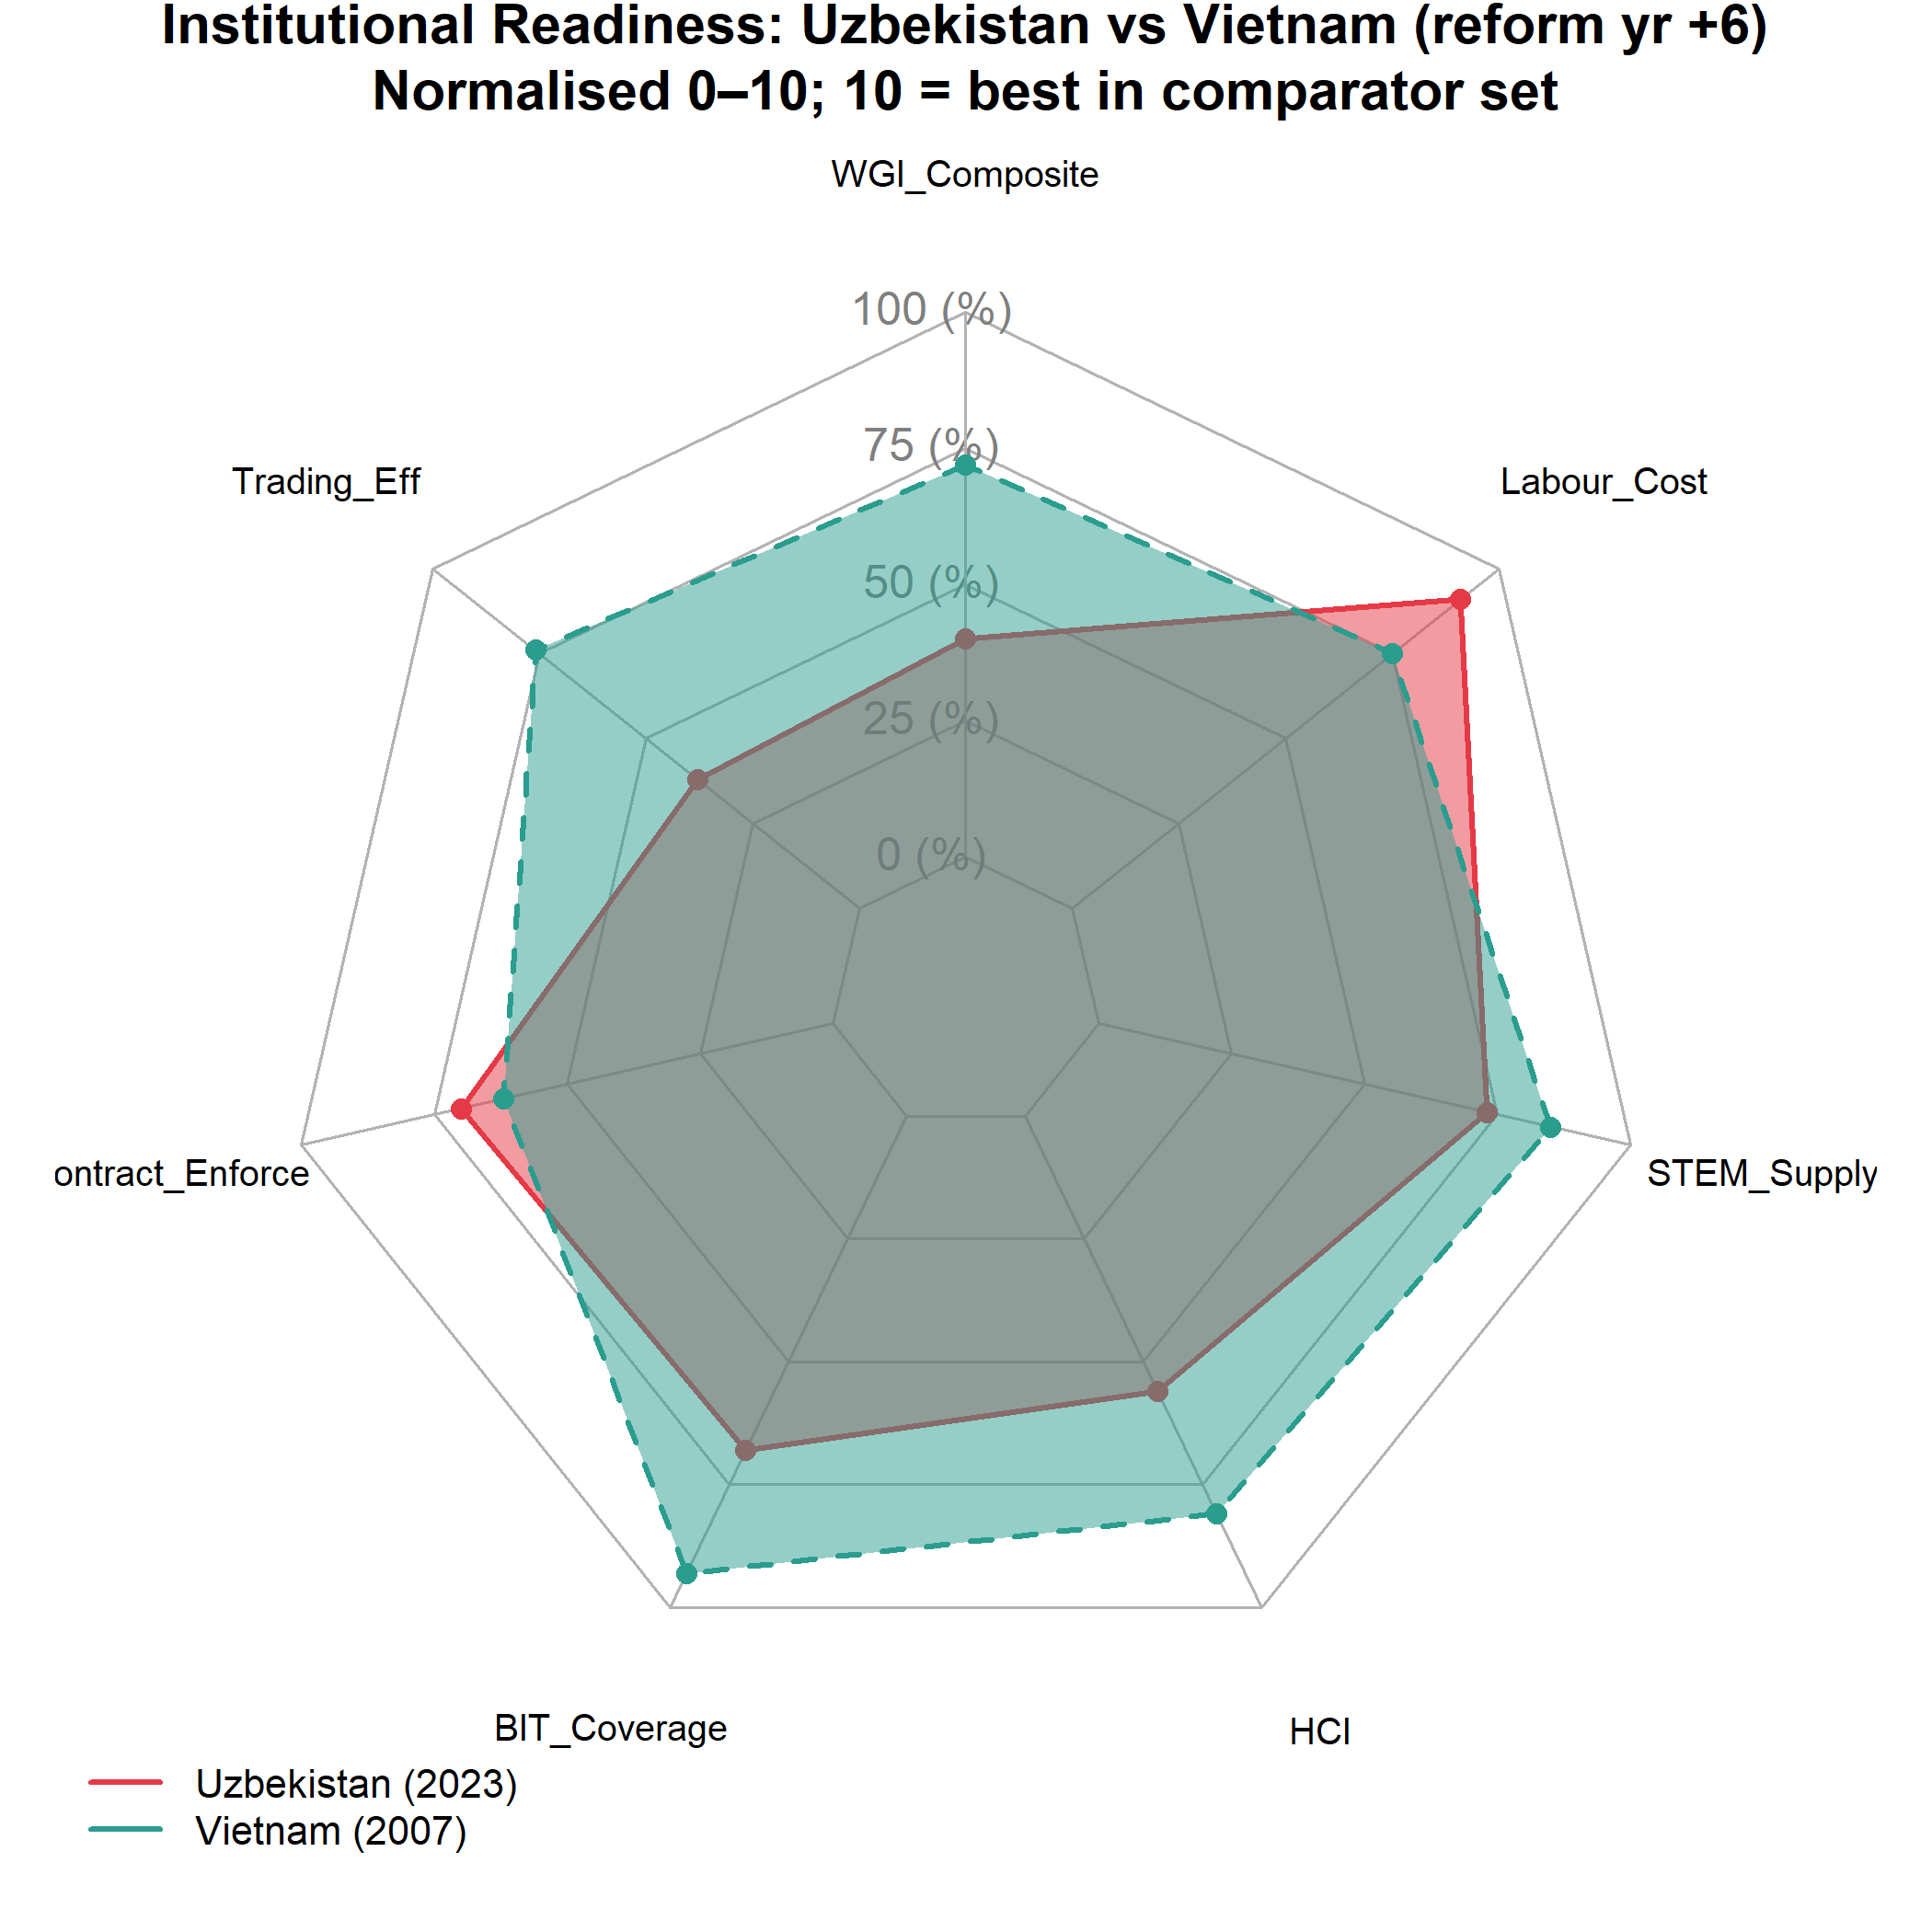
\includegraphics[width=0.70\textwidth]{figures/fig19_institutional_radar.png}
 \caption{Institutional Readiness Radar: Uzbekistan vs.\ Vietnam at Reform Year +6. Scores normalised 0--10; 10 = best in comparator set. Dimensions: WGI Composite, Trading Efficiency, Contract Enforcement, BIT Coverage, HCI, STEM Supply, Labour Cost. Source: World Bank, UNCTAD, ILO; author calculations.}
 \label{fig:institutional_radar}
\end{figure}

Uzbekistan scores competitively on Labour Cost and STEM Supply relative to Vietnam, and favourably on Trading Efficiency's contract-enforcement dimension. The most significant deficits are in WGI Composite (governance quality) and Trading Efficiency (border crossing time). These dimensions map directly onto the type of GVC upgrade needed: from captive (infrastructure, resource extraction) to relational (technology-intensive manufacturing), which requires precisely the governance quality and trade facilitation speed that Uzbekistan currently under-delivers relative to its comparators.
